

\tikzset{every picture/.style={line width=0.75pt}} %set default line width to 0.75pt        

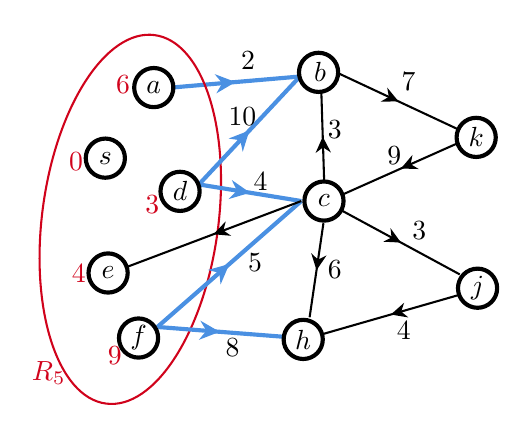
\begin{tikzpicture}[x=0.5pt,y=0.5pt,yscale=-1,xscale=1]
%uncomment if require: \path (0,296); %set diagram left start at 0, and has height of 296

%Straight Lines [id:da3320252336737717] 
\draw [color={rgb, 255:red, 74; green, 144; blue, 226 }  ,draw opacity=1 ][line width=1.5]    (119,48) -- (212,40) ;
\draw [shift={(165.5,44)}, rotate = 535.0799999999999] [fill={rgb, 255:red, 74; green, 144; blue, 226 }  ,fill opacity=1 ][line width=0.08]  [draw opacity=0] (14.56,-6.99) -- (0,0) -- (14.56,6.99) -- (9.67,0) -- cycle    ;
%Shape: Ellipse [id:dp2857420369455096] 
\draw  [color={rgb, 255:red, 208; green, 2; blue, 27 }  ,draw opacity=1 ] (26.24,134.88) .. controls (35.95,61.34) and (72.1,5.46) .. (106.98,10.07) .. controls (141.87,14.67) and (162.28,78.02) .. (152.57,151.56) .. controls (142.86,225.1) and (106.71,280.98) .. (71.83,276.37) .. controls (36.94,271.77) and (16.53,208.42) .. (26.24,134.88) -- cycle ;
%Straight Lines [id:da02943457575339692] 
\draw [color={rgb, 255:red, 74; green, 144; blue, 226 }  ,draw opacity=1 ][line width=1.5]    (139,118) -- (212,40) ;
\draw [shift={(175.5,79)}, rotate = 493.1] [fill={rgb, 255:red, 74; green, 144; blue, 226 }  ,fill opacity=1 ][line width=0.08]  [draw opacity=0] (14.56,-6.99) -- (0,0) -- (14.56,6.99) -- (9.67,0) -- cycle    ;
%Straight Lines [id:da7032022658079198] 
\draw [color={rgb, 255:red, 74; green, 144; blue, 226 }  ,draw opacity=1 ][line width=1.5]    (139,118) -- (213,130) ;
\draw [shift={(176,124)}, rotate = 189.21] [fill={rgb, 255:red, 74; green, 144; blue, 226 }  ,fill opacity=1 ][line width=0.08]  [draw opacity=0] (14.56,-6.99) -- (0,0) -- (14.56,6.99) -- (9.67,0) -- cycle    ;
%Straight Lines [id:da9416797747261806] 
\draw [color={rgb, 255:red, 74; green, 144; blue, 226 }  ,draw opacity=1 ][line width=1.5]    (109,221) -- (213,130) ;
\draw [shift={(161,175.5)}, rotate = 498.81] [fill={rgb, 255:red, 74; green, 144; blue, 226 }  ,fill opacity=1 ][line width=0.08]  [draw opacity=0] (14.56,-6.99) -- (0,0) -- (14.56,6.99) -- (9.67,0) -- cycle    ;
%Straight Lines [id:da6197316893700862] 
\draw [color={rgb, 255:red, 74; green, 144; blue, 226 }  ,draw opacity=1 ][line width=1.5]    (109,221) -- (199,228) ;
\draw [shift={(154,224.5)}, rotate = 184.45] [fill={rgb, 255:red, 74; green, 144; blue, 226 }  ,fill opacity=1 ][line width=0.08]  [draw opacity=0] (14.56,-6.99) -- (0,0) -- (14.56,6.99) -- (9.67,0) -- cycle    ;
%Straight Lines [id:da7705917014251779] 
\draw [color={rgb, 255:red, 0; green, 0; blue, 0 }  ,draw opacity=1 ][line width=0.75]    (86,178) -- (213,130) ;
\draw [shift={(149.5,154)}, rotate = 339.3] [fill={rgb, 255:red, 0; green, 0; blue, 0 }  ,fill opacity=1 ][line width=0.08]  [draw opacity=0] (11.61,-5.58) -- (0,0) -- (11.61,5.58) -- (7.71,0) -- cycle    ;
%Straight Lines [id:da7178806242260687] 
\draw [color={rgb, 255:red, 0; green, 0; blue, 0 }  ,draw opacity=1 ][line width=0.75]    (326,78) -- (240.5,38) ;
\draw [shift={(283.25,58)}, rotate = 205.07] [fill={rgb, 255:red, 0; green, 0; blue, 0 }  ,fill opacity=1 ][line width=0.08]  [draw opacity=0] (11.61,-5.58) -- (0,0) -- (11.61,5.58) -- (7.71,0) -- cycle    ;
%Straight Lines [id:da2873203830948724] 
\draw [color={rgb, 255:red, 0; green, 0; blue, 0 }  ,draw opacity=1 ][line width=0.75]    (326.5,88) -- (243.5,125) ;
\draw [shift={(285,106.5)}, rotate = 335.97] [fill={rgb, 255:red, 0; green, 0; blue, 0 }  ,fill opacity=1 ][line width=0.08]  [draw opacity=0] (11.61,-5.58) -- (0,0) -- (11.61,5.58) -- (7.71,0) -- cycle    ;
%Straight Lines [id:da9325647569597147] 
\draw [color={rgb, 255:red, 0; green, 0; blue, 0 }  ,draw opacity=1 ][line width=0.75]    (327.5,183) -- (242.5,137) ;
\draw [shift={(285,160)}, rotate = 208.42] [fill={rgb, 255:red, 0; green, 0; blue, 0 }  ,fill opacity=1 ][line width=0.08]  [draw opacity=0] (11.61,-5.58) -- (0,0) -- (11.61,5.58) -- (7.71,0) -- cycle    ;
%Straight Lines [id:da8240281406202591] 
\draw [color={rgb, 255:red, 0; green, 0; blue, 0 }  ,draw opacity=1 ][line width=0.75]    (219,214) -- (229,146) ;
\draw [shift={(224,180)}, rotate = 278.37] [fill={rgb, 255:red, 0; green, 0; blue, 0 }  ,fill opacity=1 ][line width=0.08]  [draw opacity=0] (11.61,-5.58) -- (0,0) -- (11.61,5.58) -- (7.71,0) -- cycle    ;
%Straight Lines [id:da6386544223700206] 
\draw [color={rgb, 255:red, 0; green, 0; blue, 0 }  ,draw opacity=1 ][line width=0.75]    (229,226) -- (326.5,198) ;
\draw [shift={(277.75,212)}, rotate = 343.98] [fill={rgb, 255:red, 0; green, 0; blue, 0 }  ,fill opacity=1 ][line width=0.08]  [draw opacity=0] (11.61,-5.58) -- (0,0) -- (11.61,5.58) -- (7.71,0) -- cycle    ;
%Straight Lines [id:da7268529078901531] 
\draw [color={rgb, 255:red, 0; green, 0; blue, 0 }  ,draw opacity=1 ][line width=0.75]    (229.5,115) -- (227.5,52) ;
\draw [shift={(228.5,83.5)}, rotate = 448.18] [fill={rgb, 255:red, 0; green, 0; blue, 0 }  ,fill opacity=1 ][line width=0.08]  [draw opacity=0] (11.61,-5.58) -- (0,0) -- (11.61,5.58) -- (7.71,0) -- cycle    ;

% Text Node
\draw (16,244) node [anchor=north west][inner sep=0.75pt]   [align=left] {$\displaystyle \textcolor[rgb]{0.82,0.01,0.11}{R}\textcolor[rgb]{0.82,0.01,0.11}{_{5}}$};
% Text Node
\draw (43,93) node [anchor=north west][inner sep=0.75pt]   [align=left] {$\displaystyle \textcolor[rgb]{0.82,0.01,0.11}{0}$};
% Text Node
\draw (167.24,20.06) node [anchor=north west][inner sep=0.75pt]   [align=left] {$\displaystyle 2$};
% Text Node
\draw  [line width=1.5]   (71.38, 99) circle [x radius= 14.15, y radius= 14.15]   ;
\draw (71.38,99) node   [align=left] {$\displaystyle s$};
% Text Node
\draw (77,37) node [anchor=north west][inner sep=0.75pt]   [align=left] {$\displaystyle \textcolor[rgb]{0.82,0.01,0.11}{6}$};
% Text Node
\draw  [line width=1.5]   (106.38, 48) circle [x radius= 14.15, y radius= 14.15]   ;
\draw (106.38,48) node   [align=left] {$\displaystyle a$};
% Text Node
\draw (98,124) node [anchor=north west][inner sep=0.75pt]   [align=left] {$\displaystyle \textcolor[rgb]{0.82,0.01,0.11}{3}$};
% Text Node
\draw  [line width=1.5]   (125.38, 123) circle [x radius= 14.15, y radius= 14.15]   ;
\draw (125.38,123) node   [align=left] {$\displaystyle d$};
% Text Node
\draw (45,174) node [anchor=north west][inner sep=0.75pt]   [align=left] {$\displaystyle \textcolor[rgb]{0.82,0.01,0.11}{4}$};
% Text Node
\draw  [line width=1.5]   (73.38, 182) circle [x radius= 14.15, y radius= 14.15]   ;
\draw (73.38,182) node   [align=left] {$\displaystyle e$};
% Text Node
\draw  [line width=1.5]   (225.48, 37) circle [x radius= 14.15, y radius= 14.15]   ;
\draw (219.98,37) node [anchor=west] [inner sep=0.75pt]   [align=left] {$\displaystyle b$};
% Text Node
\draw  [line width=1.5]   (229.38, 130) circle [x radius= 14.15, y radius= 14.15]   ;
\draw (229.38,130) node   [align=left] {$\displaystyle c$};
% Text Node
\draw  [line width=1.5]   (339.38, 84) circle [x radius= 14.15, y radius= 14.15]   ;
\draw (339.38,84) node   [align=left] {$\displaystyle k$};
% Text Node
\draw  [line width=1.5]   (214.38, 230) circle [x radius= 14.15, y radius= 14.15]   ;
\draw (214.38,230) node   [align=left] {$\displaystyle h$};
% Text Node
\draw (71,233) node [anchor=north west][inner sep=0.75pt]   [align=left] {$\displaystyle \textcolor[rgb]{0.82,0.01,0.11}{9}$};
% Text Node
\draw  [line width=1.5]   (95.38, 229) circle [x radius= 14.15, y radius= 14.15]   ;
\draw (95.38,229) node   [align=left] {$\displaystyle f$};
% Text Node
\draw  [line width=1.5]   (340.38, 193) circle [x radius= 14.15, y radius= 14.15]   ;
\draw (340.38,193) node   [align=left] {$\displaystyle j$};
% Text Node
\draw (158.24,60.06) node [anchor=north west][inner sep=0.75pt]   [align=left] {$\displaystyle 10$};
% Text Node
\draw (176.24,107.06) node [anchor=north west][inner sep=0.75pt]   [align=left] {$\displaystyle 4$};
% Text Node
\draw (172.24,166.06) node [anchor=north west][inner sep=0.75pt]   [align=left] {$\displaystyle 5$};
% Text Node
\draw (156,227.5) node [anchor=north west][inner sep=0.75pt]   [align=left] {$\displaystyle 8$};
% Text Node
\draw (283.24,35.06) node [anchor=north west][inner sep=0.75pt]   [align=left] {$\displaystyle 7$};
% Text Node
\draw (291,143) node [anchor=north west][inner sep=0.75pt]   [align=left] {$\displaystyle 3$};
% Text Node
\draw (279.75,215) node [anchor=north west][inner sep=0.75pt]   [align=left] {$\displaystyle 4$};
% Text Node
\draw (273,88.47) node [anchor=north west][inner sep=0.75pt]   [align=left] {$\displaystyle 9$};
% Text Node
\draw (230,70) node [anchor=north west][inner sep=0.75pt]   [align=left] {$\displaystyle 3$};
% Text Node
\draw (230,171) node [anchor=north west][inner sep=0.75pt]   [align=left] {$\displaystyle 6$};


\end{tikzpicture}

